\documentclass{article}
\usepackage[margin=1.4in]{geometry}
\usepackage[brazil]{babel}
\usepackage[utf8]{inputenc}
\usepackage{amsmath}
\usepackage{indentfirst}
\usepackage{cite}
\usepackage{url}
\usepackage{graphics}
\usepackage{graphicx}
\usepackage{caption}
\usepackage{subcaption}
\usepackage{multirow}
\usepackage{amsfonts}

\title{Geração de Grid - Funções de Controle}
\author{Rafael Umino Nakanishi}

\date{}

\newcommand{\diff}[2]{
	\frac{\partial #1}{\partial #2}
}
\newcommand{\diffxixi}[1]{
	\diff{#1}{\xi^2}
}
\newcommand{\diffetaeta}[1]{
	\diff{#1}{\eta^2}
}
\newcommand{\diffxieta}[1]{
	\diff{^2#1}{\xi\partial\eta}
}
\newcommand{\diffxi}[1]{
	\diff{#1}{\xi}
}
\newcommand{\diffeta}[1]{
	\diff{#1}{\eta}
}

\begin{document}
	\maketitle

	\section{Objetivo} % (fold)
	\label{sec:objetivo}
		O objetivo desse trabalho foi desenvolver as técnicas de geração da grid baseados em métodos diferenciais elípticos. Nessas técnicas, a malha é gerada através das soluções de Equações Diferenciais Parciais elípticas. Os geradores de malhas mais utilizados são os pares de equação de Laplace:
		\begin{eqnarray}
			\nabla^2\xi = 0 \text{  e  } \nabla^2\eta = 0 
		\end{eqnarray}

		Tal sistema possui uma características desejáveis, incluindo o princípio do máximo, que garante que nem o máximo nem o mínimo de $\xi, \eta$ ocorram no inerior do domínio. Além disso, é garantido que se as fronteiras do domínio variam de forma suave e monótona, então o interior da malha também terá essa característica.
	% section objetivo (end)

		\subsection{Método de TTM} % (fold)
		\label{sec:ttm-method}
			Em alguns casos, é desejado ainda que certas regiões da malha sejam mais refinados que as demais partes. Para isso faz-se uso das equações de Poisson:
			\begin{eqnarray}
				\nabla^2\xi = P(\xi, \eta) \text{  e  } \nabla^2\eta = Q(\xi, \eta) \label{eqn:poisson}
			\end{eqnarray}
			onde $P(\xi,\eta)$ e $Q(\xi,\eta)$ são chamdas funções de controle. É possível demonstrar que as equações do problema inverso são dadas por:
			\begin{eqnarray}
			\label{eqn:ttm}
				g_{22}\diffxixi{x} - 2g_{12}\diffxieta{x} + g_{11}\diffetaeta{x} + g \Big(P\diffxi{x}+Q\diffeta{x}\Big)\\ \nonumber
				g_{22}\diffxixi{y} - 2g_{12}\diffxieta{y} + g_{11}\diffetaeta{y} + g \Big(P\diffxi{y}+Q\diffeta{y}\Big)
			\end{eqnarray}

			De fato, tomando as relações a seguir:
			\begin{eqnarray*}
				\left\{
				\begin{array}{l l}
					\nabla\cdot u(x^1, x^2) &= \diff{u}{x^i}g^i\\
					\nabla f(x^1, x^2) &= g^i\diff{f}{x^i}
				\end{array} \right.
			\end{eqnarray*}
			é pośsível mostrar que:
			\begin{eqnarray*}
				\Delta x^i = \nabla\cdot\nabla x^i = g^k \frac{\partial}{\partial x^k}\Big( g^j \diff{x^i}{x^j} \Big) \nonumber
			\end{eqnarray*}
			Observe que $\diff{x^i}{x^j} = \delta^i_j$. Aplicando contração de índice, onde $g^j\delta^i_j = g^i$, e a definição do símbolo de Christoffel, temos:
			\begin{eqnarray*}
				\Delta x^i &=& g^k \diff{g^i}{x^k} \\ \nonumber
				 &=& g^k (-\Gamma^i_{kj} g^j)\\ \nonumber 
				 &=& -g^{kj}\Gamma^i_{kj} \nonumber
 			\end{eqnarray*}
 			Aplicando uma das propriedades do símbolo de Christoffel, chegamos a:
 			\begin{eqnarray}
 				\Delta x^i = -g^{kj}\Big( \diff{^2y_k}{x^j\partial x^k} \diff{x^i}{ y_l} \Big)
 			\end{eqnarray}
 			Multiplicando ambos os termos da expressão acima por $\diff{y_ l}{x^i}$, obtemos finalmente:
 			\begin{eqnarray}
 				\Delta x^i \diff{y_ l}{x^i} = -g^{kj}  \diff{^2y_k}{x^j\partial x^k }
 			\end{eqnarray}
 			E aplicando as coordenadas $(x^1, x^2) = (\xi, \eta)$ e $(y_1,y_2) = (x,y)$ obtemos a equação (segue análogo para $y$):
 			\begin{eqnarray}
 				\Delta\xi \diffxi{x} + \Delta\eta\diffeta{x} = - \Big(g^{11}\diffxixi{x} + 2g^{12}\diffxieta{x} + g^{22}\diffetaeta{x}\Big)\label{eqn:final}
 			\end{eqnarray}

 			Note que $g^{ij}$ mapeia das coordenadas curvilpíneas para as coordenadas cartesianas. Como queremoso efeito contrário, encontremos $g_{ij}$:
 			\begin{eqnarray}\label{eqn:tensor}
	 			\begin{bmatrix}
	 				g^{11} & g^{12}\\
	 				g^{12} & g^{22}	
	 			\end{bmatrix}
	 			=
	 			\frac{1}{g}
	 			\begin{bmatrix}
	 				g_{22} & -g_{12}\\
	 				-g_{12} & g_{11}
	 			\end{bmatrix}
 			\end{eqnarray}
 			E substituindo as Equãções \ref{eqn:poisson} e \ref{eqn:tensor} na Equação \ref{eqn:final} obtemos as equações do método TTM (Thomson, Thames, Mastin) (Eq. \ref{eqn:ttm}).
		% section ttm-method (end)

	\section{Técnicas Numéricas} % (fold)
	\label{sec:t_cnicas_num_ricas}

		Apresentamos nas subseções seguintes as discretizações que foram utilizadas para resolução numérica do problema e como foi feita a escolha dos valores iniciais utilizados.

		\subsection{Discretização} % (fold)
		\label{sub:discretiza_o}
			As principais discretizações realizadas foram feitas por diferenças finitas. Listamos a seguir as discretizações dos tensores métricos e das derivadas parciais de $x$ e $y$.

			\begin{eqnarray*}
				g_{11} = \Bigg[ \Big( \diffxi{x}^2 \Big) + \Big(\diffxi{y}\Big)^2 \Bigg] &=& \Big( \frac{x_{i+1,j} - x_{i-1,j}}{2\Delta\xi} \Big)^2 + \Big( \frac{y_{i+1,j} - y_{i-1,j}}{2\Delta\xi} \Big)^2\\
				g_{22} = \Bigg[ \Big( \diffeta{x}^2 \Big) + \Big(\diffeta{y}\Big)^2 \Bigg] &=& \Big( \frac{x_{i,j+1} - x_{i,j-1}}{2\Delta\eta} \Big)^2 + \Big( \frac{y_{i,j+1} - y_{i,j-1}}{2\Delta\eta} \Big)^2
			\end{eqnarray*}
			\begin{multline*}
				g_{12} = \Bigg[ \Big( \diffxi{x}\Big)\Big(\diffeta{x} \Big) + \Big(\diffxi{y}\Big)\Big(\diffeta{y}\Big) \Bigg] = \\
					= \Big( \frac{x_{i,j+1} - x_{i,j-1}}{2\Delta\eta} \Big) \Big( \frac{x_{i,j+1} - x_{i,j-1}}{2\Delta\eta} \Big) + \Big( \frac{y_{i,j+1} - y_{i,j-1}}{2\Delta\eta} \Big)\Big( \frac{y_{i+1,j} - y_{i-1,j}}{2\Delta\xi} \Big)
			\end{multline*}

			Destacamos, também as diferenças finitas utilizadas para as segunda derivadas de $x$ (seguindo as equações a seguir análogas para $y$):

			\begin{eqnarray*}
				\Big( \diffxixi{x} \Big) &=& \frac{x_{i+1,j} - 2x_{i,j} + x_{i-1,j}}{(\Delta\xi)^2}\\
				\Big( \diffetaeta{x} \Big) &=& \frac{x_{i,j+1} - 2x_{i,j} + x_{i,j-1}}{(\Delta\eta)^2}\\
				\Big( \diffxieta{x} \Big) &=& \frac{x_{i+1,j+1} +x_{i-1,j-1} - x_{i-1,j+1} - x_{i+1,j-1}}{4(\Delta\xi)(\Delta\eta)}
			\end{eqnarray*}
		% subsection discretiza_o (end)

		\subsection{Interpolação Transfinita} % (fold)
		\label{sub:interpola_o_transfinita}
			Para geração dos pontos iniciais na malha, foi utilizado o método de interpolação transfinita. Tal método permite manter a curvatura do domínio físico e gera uma malha de modo rápido e simples. Observe na figura COLOQUE UMA FIGURA que o mapeamento é feito de forma a manter as fronteiras do domínio original.

			Para a interpolação fazemos uso de projetores $\mathbf{P}_{\xi}(\xi, \eta) = (1-\xi)\mathbf{r}(0,\eta) + \xi\mathbf{r}(1,\eta)$ e $\mathbf{P}_{\eta}(\xi, \eta) = (1-\eta)\mathbf{r}(\xi,0) + \eta\mathbf{r}(\xi,1)$. Utilizado esse projetores é possível preservar os vértices, mas não a fronteira. Então, compondo os projetores mencionados, em uma soma booleana, temos:
			\begin{eqnarray*}
				\mathbf{P}_\xi \oplus \mathbf{P}_\eta(\xi, \eta) &=& \mathbf{P}_\xi + \mathbf{P}_\eta - \mathbf{P}_\xi\mathbf{P}_\eta \\
						 &=& (1-\xi)\mathbf{r}(0,\eta) + \xi\mathbf{r}(1,\eta) + (1-\eta)\mathbf{r}(\xi,0) + \eta\mathbf{r}(\xi,1)\\
						&&- (1-\xi)(1-\eta)\mathbf{r}(0,0) - (1-\xi)\eta\mathbf{r}(0,1)\\
						&&- (1-\eta)\xi\mathbf{r}(1,0) - \xi\eta\mathbf{r}(1,1)
			\end{eqnarray*}

			Melhorando a escrita da equação acima, escrevemos:
			\begin{eqnarray*}
						\mathbf{r}(\xi,\eta)&=& (1-\xi)\mathbf{r}_l(\eta) + \xi\mathbf{r}_r(\eta) + (1-\eta)\mathbf{r}_b(\xi) + \eta\mathbf{r}_l(\xi) - (1-\xi)(1-\eta)\mathbf{r}_b(0) - \\
						&&(1-\xi)\eta\mathbf{r}_l(0) - (1-\eta)\xi\mathbf{r}_b(1) - \xi\eta\mathbf{r}_l(1)
			\end{eqnarray*}
			onde $t,b,l,r$ são abreviações americanas para \emph{top, bottom, left, right} respectivamente.
		% subsection interpola_o_transfinita (end)

		\subsection{Funções de Controle} % (fold)
		\label{sub:fun_es_de_controle}
			Um conjunto de funções de controle foi proposto por Thomson, Thames e Martin em 1974 e pode ser encontrado em \cite{farrashkhalvat2003basic} e transcrito a seguir:
			\begin{eqnarray}
				P(\xi,\eta) = -\sum_{n=1}^N a_n \frac{(\xi - \xi_n)}{|\xi - \xi_n|}e^{-c_n |\xi-\xi_n|} - \sum_{l=1}^{L}b_l \frac{(\xi - \xi_l)}{|\xi - \xi_l|}e^{-d_l [(\xi-\xi_l)^2 + (\eta-\eta_l)^2]^{1/2}} \\
				Q(\xi,\eta) = -\sum_{n=1}^N a_n \frac{(\eta - \eta_n)}{|\eta - \eta_n|}e^{-c_n |\eta-\eta_n|} - \sum_{l=1}^{L}b_l \frac{(\eta - \eta_l)}{|\eta - \eta_l|}e^{-d_l [(\xi-\xi_l)^2 + (\eta-\eta_l)^2]^{1/2} }
			\end{eqnarray}

			Note que $N$ é o número de linhas e $L$ é o número de pontos para onde a malha será atraída, ou seja, onde haverá maior refinamento. Além disso, os coeficientes $a_n, c_n, b_l, d_l$ são positivos. O primeiro termo da expressão $P(\xi,\eta)$ tem o efeito, com amplitude $a_n$, de atrair linhas onde $\xi$ é constante para as curvas $\xi = \xi_n$ no domínio físico. Enquanto o segundo termo da expressão, com amplitude $b_l$, tem o efeito de atrair as linhas $\xi$ para os pontos $(\xi_l, \eta_l)$.
		% subsection fun_es_de_controle (end)
	% section t_cnicas_num_ricas (end)

	\section{Detalhes de Implementação} % (fold)
	\label{sec:detalhes_de_implementa_o}
		Em soluções numéricas a serem utilizadas para resolução de sistemas diferenciais, diferenças finitas frequentemente envolvem equações que geram um sistema de matriz tridiagonal. Com isso, podemos apresentar os métodos de elminação de Gauss: Jacobi, Gauss-Seidel, SOR(Successive Over Relaxation) e Thomas.

		Vale ressaltar que os valores iniciais utilizados foram gerados utilizando-se interpolação transfinita, apresentada anteriormente.

		Discutimos a seguir os detalhes de implementação pertinentes às técnicas implementadas.

		\subsection{Método de Jacobi, Gauss Seidel e SOR} % (fold)
		\label{sub:m_todo_de_jacobi}
			Os métodos de Jacobi, Gauss Seidel e SOR são bem semelhantes e optamos por explicá-los em conjunto.

			\subsubsection{Método Jacobi} % (fold)
			\label{ssub:m_todo_jacobi}
				Para o método de Jacobi foi necessário criar uma matriz auxiliar para armazenamento dos valores da iteração corrente. Essa abordagem é própria do método, já que faz uso dos valores da iteração anterior para cálculo dos novos valores. Em termos simples, temos que o método de Jacobi pode ser escrito como:
				\begin{eqnarray*}
					x_i^{(k)} = \sum_{j=1}^N a_{ij}x_j^{(k-1)}
				\end{eqnarray*}
				onde $k$ é o valor da iteração corrente.
			% subsubsection m_todo_jacobi (end)

			\subsubsection{Método de Gauss Seidel} % (fold)
			\label{ssub:m_todo_de_gauss_seidel}
				A criação de uma nova matriz não se faz necessária no método de Gauss Seidel, uma vez que os valores já calculados podem ser utilizados na iteração corrente. Além disso é possível notar uma certa aceleração do método. Podemos descrever o método de Gauss Seidel, em termos simples, como sendo:
				\begin{eqnarray*}
					x_i^{(k)} = \sum_{j=1}^{i-1} a_{ij}x_j^(k) + \sum_{j=i+1}^{N} a_{ij}x_j^{(k-1)}
				\end{eqnarray*}
			% subsubsection m_todo_de_gauss_seidel (end)

			\subsubsection{Método SOR} % (fold)
			\label{ssub:m_todo_sor}
				O método de SOR é baseado no método de Gauss Seidel e são utilizados para acelerar a convergência de sistemas que convergem com o método de Gauss. Podemos, então reescrever o método de Gauss da seguinte forma:
				\begin{eqnarray}
					x_i^{(k)} = (1-\omega) x_i^{(k)}  + \omega \Bigg[\sum_{j=1}^{i-1} a_{ij}x_j^(k) + \sum_{j=i+1}^{N} a_{ij}x_j^{(k-1)} \Bigg]
				\end{eqnarray}
				onde $0 \le \omega \le 2$. \nocite{burden2008analise} 
			% subsubsection m_todo_sor (end)
		% subsection m_todo_de_jacobi (end)

		\subsection{Método de Thomas} % (fold)
		\label{sub:m_todo_de_thomas}
			Um sistema tipico a ser resolvido pelo método de Thomas, que é baseado no método de Gauss Seidel, é apresentado da forma
			\begin{eqnarray}
				-a_i u_{i-1} + b_i u_{i} - c_i u_{i+1} = d_i \label{eqn:thomas}
			\end{eqnarray}
			com $i = 1...(N-1)$ e os valores de $u_0$ e $u_N$ são supostamente conhecidos, dados as condições de contorno. Observe que os valores $a, b$ e $c$ são correspondentes à diagonal da matriz tridiagonal
			$$\begin{bmatrix}
				b_1 	& -c_1 	& 0  	&  \dots 	& 0\\
				-a_2 	& b_2 	& -c_2 	&  \dots 	& 0\\
				\vdots 	& \vdots& \ddots& \dots 	& \vdots\\
				0 		& \dots & -an_{N-2} & -b_{N-2}	& c_{N-2}\\
				0 		& \dots & \dots & -a_{N-1}	& b_{N-1}
			\end{bmatrix}$$

			Na implementação, os valores de $a,b,c,d$ podem ser derivados e obtemos os seguintes valores:
			\begin{eqnarray*}
				a_{i,j} &=& c_{i,j}  = \frac{(g_{22})_{i,j}}{(\Delta\xi)^2} - \frac{g P(i,j)}{(\Delta\xi)^2}\\
				b_{i,j} &=& \Bigg[ \frac{2(g_{22})_{i,j}}{(\Delta\xi)^2} + \frac{2(g_{11})_{i,j}}{(\Delta\eta)^2}\Bigg]\\
				d_{i,j} &=& \frac{(g_{11})_{i,j}}{(\Delta\eta)^2}(x_{i+1,j+1} + x_{i,j-1}) - 2(g_{12})_{i,j}\times\frac{x_{i+1,j+1} +x_{i-1,j-1} - x_{i-1,j+1} - x_{i+1,j-1}}{4(\Delta\xi)(\Delta\eta)} \\
					&&- g*Q(i,j)*(x_{i,j+1}-x_{i,j-1})\\
				e_{i,j} &=& \frac{(g_{11})_{i,j}}{(\Delta\eta)^2}(y_{i+1,j+1} + y_{i,j-1})- 2(g_{12})_{i,j}\times\frac{y_{i+1,j+1} +y_{i-1,j-1} - y_{i-1,j+1} - y_{i+1,j-1}}{4(\Delta\xi)(\Delta\eta)} \\
					&&- g*Q(i,j)*(y_{i,j+1}-y_{i,j-1})
			\end{eqnarray*}
			conseguindo, assim as equações da forma (\ref{eqn:thomas}), sendo $e_{i,j}$ para a variável $y$.
		% subsection m_todo_de_thomas (end)
	% section detalhes_de_implementa_o (end)

	\section{Resultados} % (fold)
	\label{sec:resultados}
		Apresentamos nessa seção os principais resultados obtidos utilizando-se as técnicas descritas anteriormente para alguns domínios físicos criados artificialmente.
		
		As Figuras (\ref{fig:ondas}-\ref{fig:m:erro}) apresentam os domínios utilizados, bem como o erro cometido a cada iteração para seus respectivos domínios. Ainda é possível observar nas figuras a quantidade de iterações que foi necessária para que os métodos convergissem. O erro tolerado nesses casos foi de $10^{-4}$.

		As Figuras (\ref{fig:ondas:ttm}-\ref{fig:m:ttm:erro}) apresentam os domínios utilizados em conjunto com funções de controle para adaptividade. Em cada figura é possível observar que os pontos da malha foram atraídos para os respectivas localizações impostas. Também é possível verificar o número de iterações necessárias para o método convergir. Observe que é necessário muito mais iterações nesses casos. O erro tolerado também foi de $10^{-4}$.

		\begin{figure}
		\centering
			\begin{subfigure}[b]{0.45\textwidth}
				\centering
				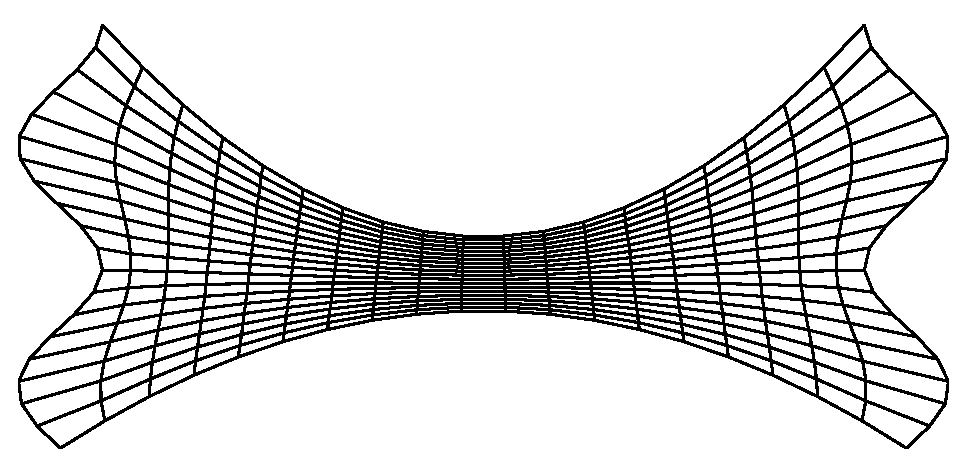
\includegraphics[width=\textwidth]{figures/waves-jacobi.eps}
				\caption{Jacobi - 264 iterações}
			\end{subfigure}
			\begin{subfigure}[b]{0.45\textwidth}
				\centering
				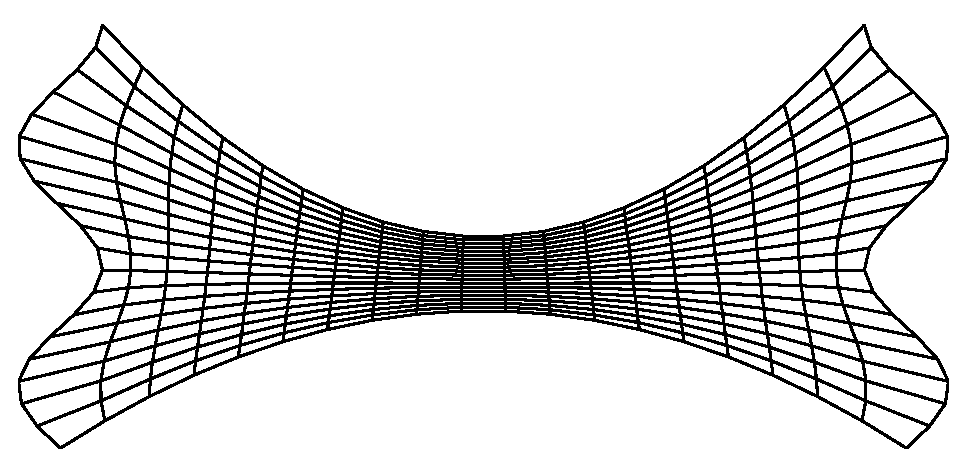
\includegraphics[width=\textwidth]{figures/waves-gauss.eps}
				\caption{Gauss-Seidel - 152 iterações}
			\end{subfigure}
			\begin{subfigure}[b]{0.45\textwidth}
				\centering
				\includegraphics[width=\textwidth]{figures/waves-sor.eps}
				\caption{SOR - 59 iterações}
			\end{subfigure}
			\begin{subfigure}[b]{0.45\textwidth}
				\centering
				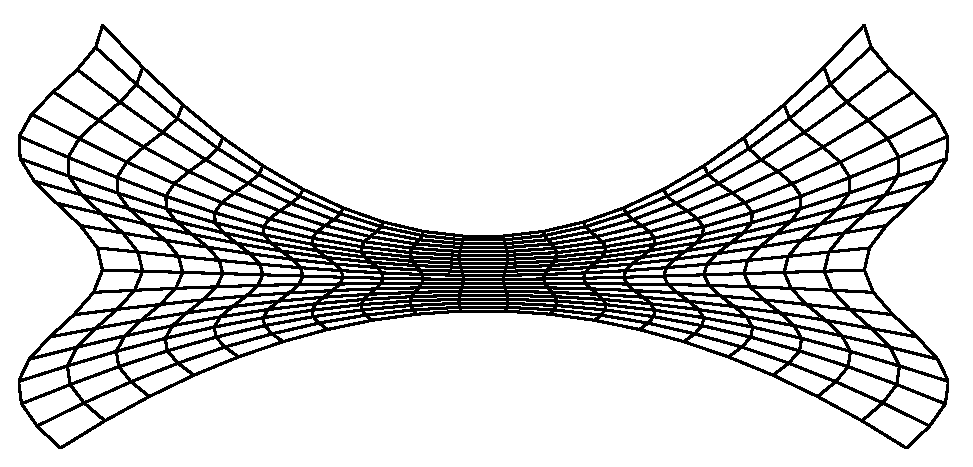
\includegraphics[width=\textwidth]{figures/waves-thomas.eps}
				\caption{Thomas - 163 iterações}
			\end{subfigure}
			\caption{Domínio ondulado}
			\label{fig:ondas}
			\centering
			\includegraphics[width=0.7\textwidth]{figures/waves-error.eps}
			\caption{Gráfico do erro para o domínio ondulado}
			\label{fig:ondas:erro}
		\end{figure}

		\begin{figure}
		\centering
			\begin{subfigure}[b]{0.45\textwidth}
				\centering
				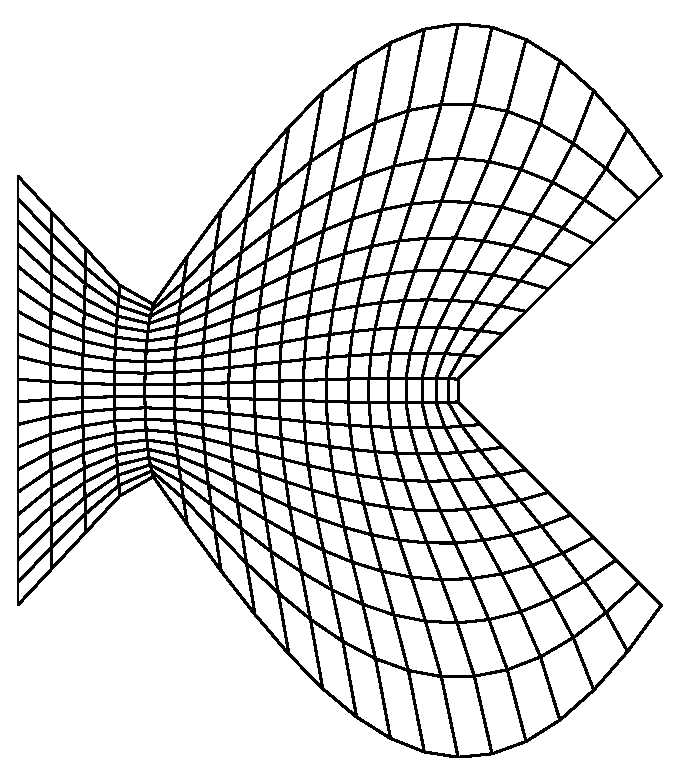
\includegraphics[width=0.6\textwidth]{figures/fish-jacobi.eps}
				\caption{Jacobi - 378 iterações}
			\end{subfigure}
			\begin{subfigure}[b]{0.45\textwidth}
				\centering
				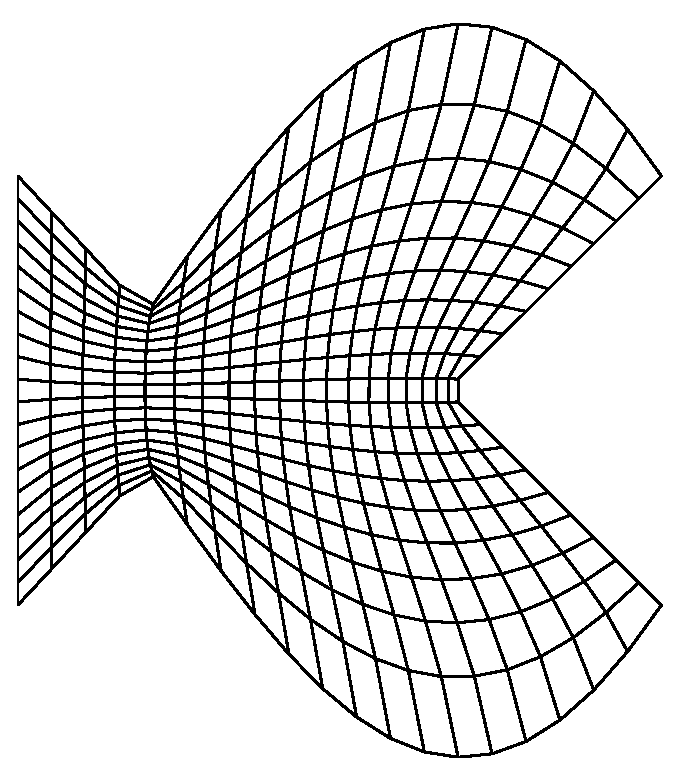
\includegraphics[width=0.6\textwidth]{figures/fish-gauss.eps}
				\caption{Gauss-Seidel - 207 iterações}
			\end{subfigure}
			\begin{subfigure}[b]{0.45\textwidth}
				\centering
				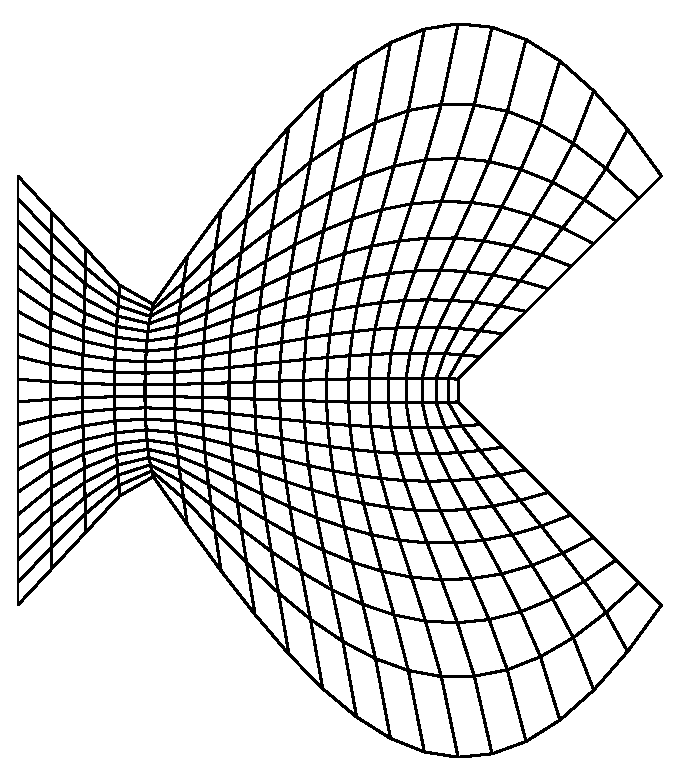
\includegraphics[width=0.6\textwidth]{figures/fish-sor.eps}
				\caption{SOR - 74 iterações}
			\end{subfigure}
			\begin{subfigure}[b]{0.45\textwidth}
				\centering
				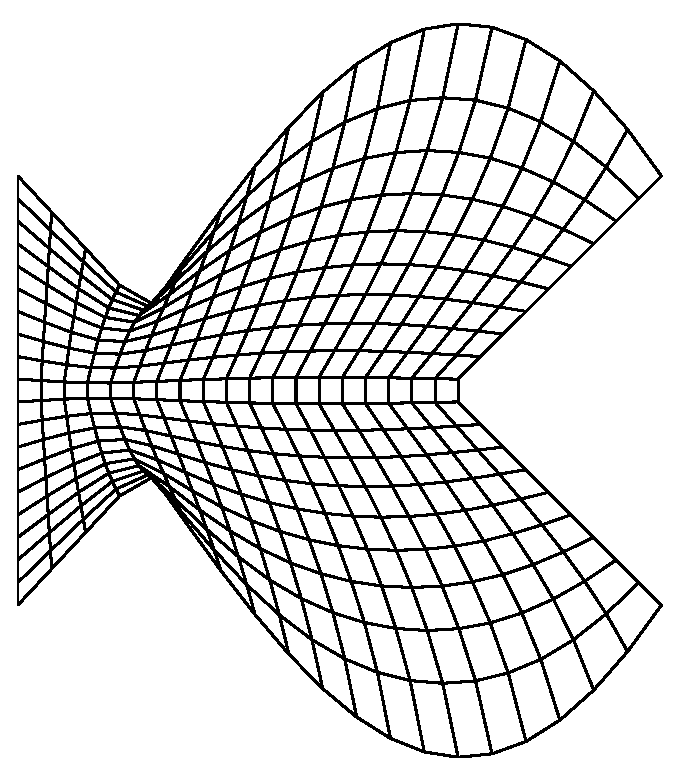
\includegraphics[width=0.6\textwidth]{figures/fish-thomas.eps}
				\caption{Thomas - 120 iterações}
			\end{subfigure}
			\caption{Domínio peixe}
			\label{fig:peixe}
			\centering
			\includegraphics[width=0.7\textwidth]{figures/fish-error.eps}
			\caption{Gráfico do erro para o domínio peixe}
			\label{fig:peixe:erro}
		\end{figure}

		\begin{figure}
		\centering
			\begin{subfigure}[b]{0.45\textwidth}
				\centering
				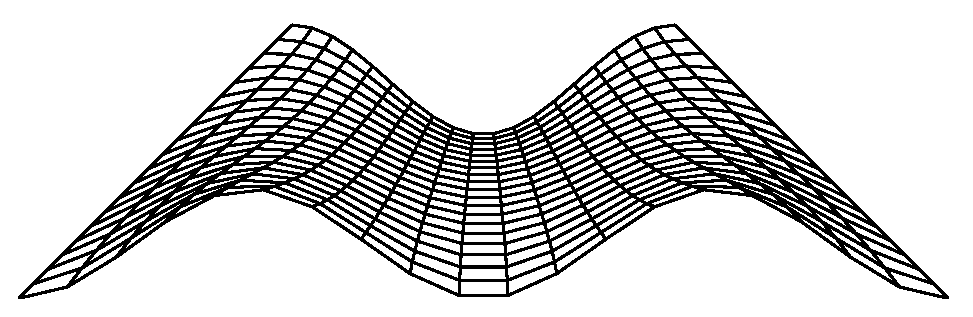
\includegraphics[width=\textwidth]{figures/m-jacobi.eps}
				\caption{Jacobi - 319 iterações}
			\end{subfigure}
			\begin{subfigure}[b]{0.45\textwidth}
				\centering
				\includegraphics[width=\textwidth]{figures/m-gauss.eps}
				\caption{Gauss-Seidel - 175 iterações}
			\end{subfigure}
			\begin{subfigure}[b]{0.45\textwidth}
				\centering
				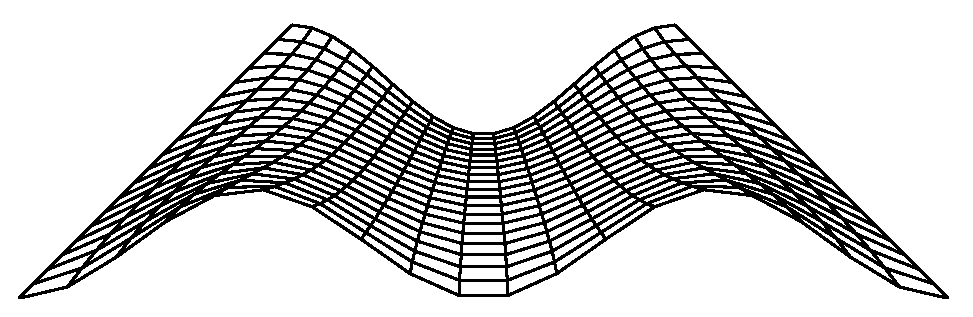
\includegraphics[width=\textwidth]{figures/m-sor.eps}
				\caption{SOR - 66 iterações}
			\end{subfigure}
			\begin{subfigure}[b]{0.45\textwidth}
				\centering
				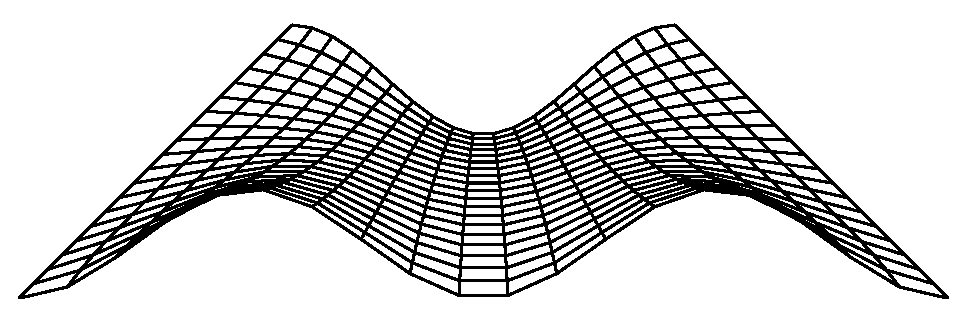
\includegraphics[width=\textwidth]{figures/m-thomas.eps}
				\caption{Thomas - 199 iterações}
			\end{subfigure}
			\caption{Domínio M}
			\label{fig:m}
			\centering
			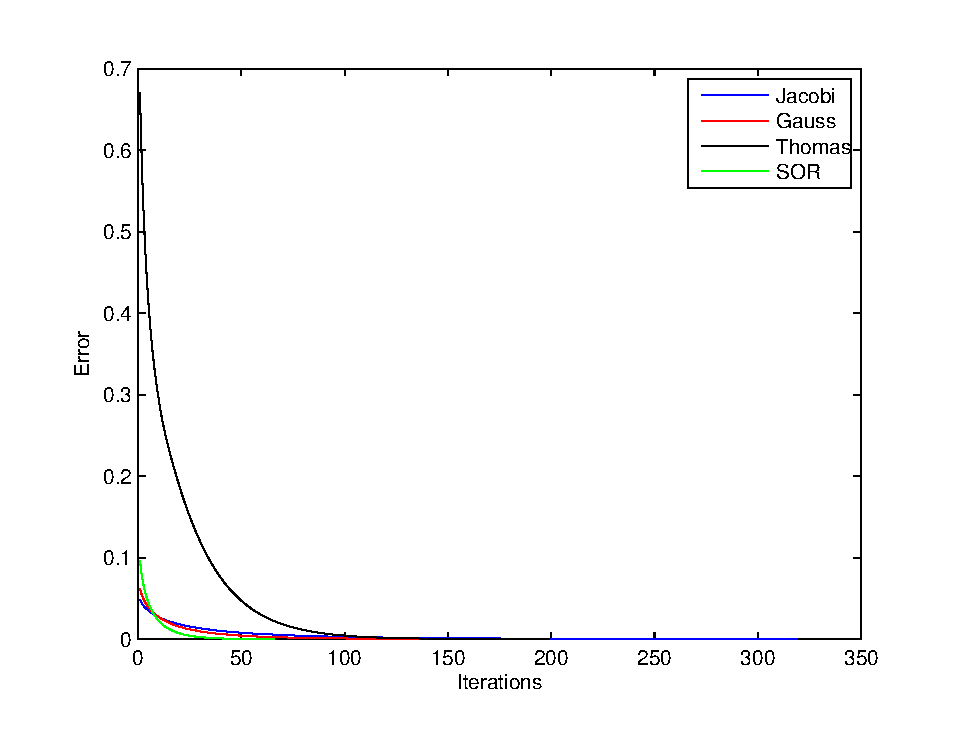
\includegraphics[width=0.7\textwidth]{figures/m-error.eps}
			\caption{Gráfico do erro para o domínio M}
			\label{fig:m:erro}
		\end{figure}

		\begin{figure}
		\centering
			\begin{subfigure}[b]{0.45\textwidth}
				\centering
				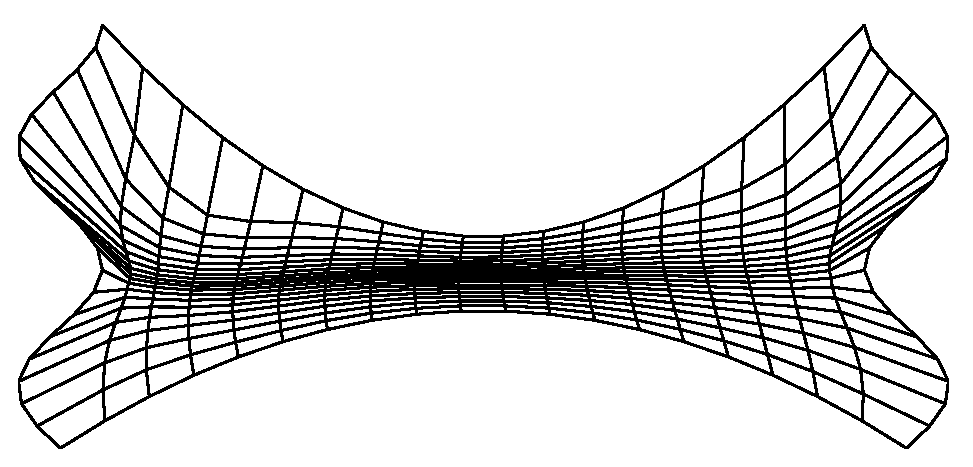
\includegraphics[width=\textwidth]{figures/waves-ttm-jacobi.eps}
				\caption{Jacobi - 915 iterações}
			\end{subfigure}
			\begin{subfigure}[b]{0.45\textwidth}
				\centering
				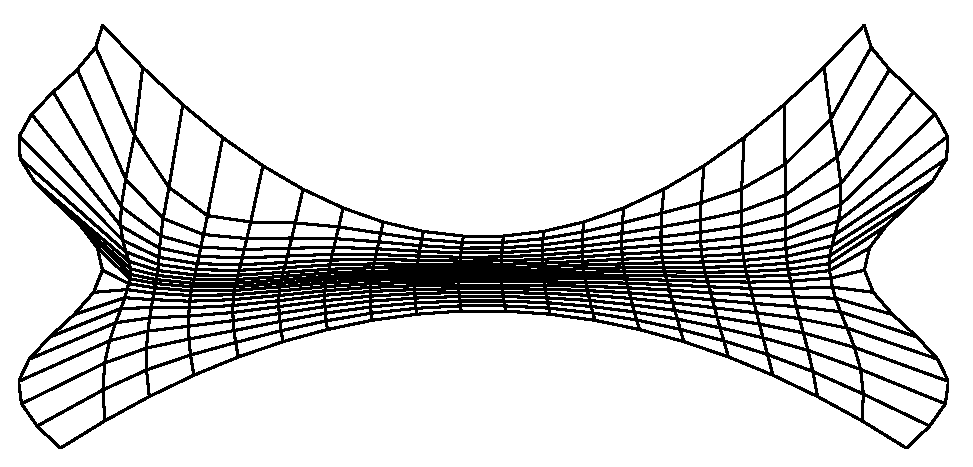
\includegraphics[width=\textwidth]{figures/waves-ttm-gauss.eps}
				\caption{Gauss-Seidel - 574 iterações}
			\end{subfigure}
			\begin{subfigure}[b]{0.45\textwidth}
				\centering
				\includegraphics[width=\textwidth]{figures/waves-ttm-sor.eps}
				\caption{SOR - 238 iterações}
			\end{subfigure}
			\caption{Domínio Ondas, aplicando o método TTM para aproximação para os pontos (0.1,0.5) e (0.9,0.5)}
			\label{fig:ondas:ttm}
			\centering
			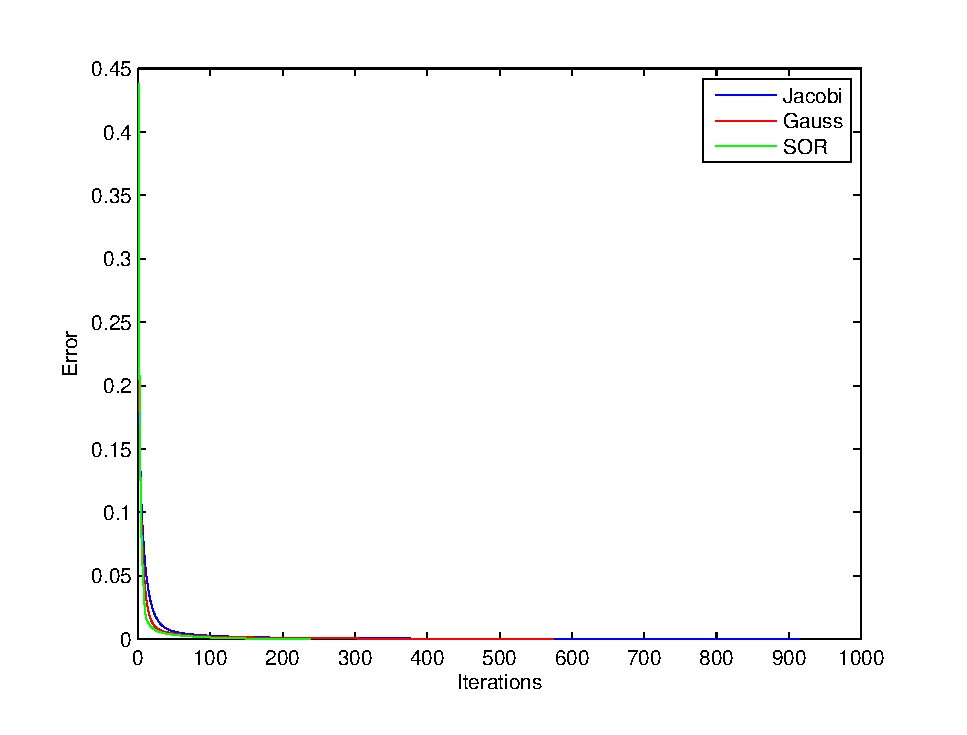
\includegraphics[width=0.7\textwidth]{figures/waves-ttm-error.eps}
			\caption{Gráfico do erro para o domínio ondas com aproximação pontual}
			\label{fig:ondas:ttm:erro}
		\end{figure}

		\begin{figure}
		\centering
			\begin{subfigure}[b]{0.45\textwidth}
				\centering
				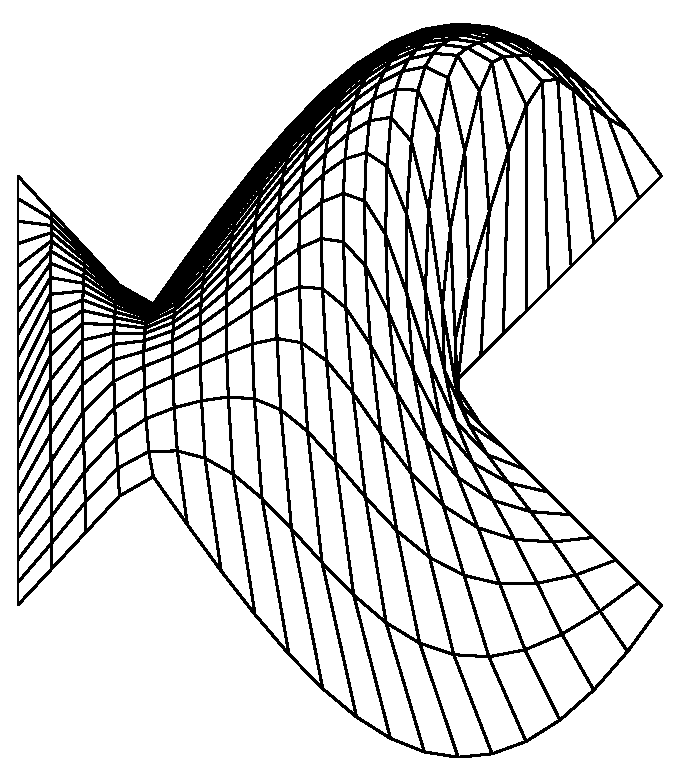
\includegraphics[width=0.7\textwidth]{figures/fish-ttm-jacobi.eps}
				\caption{Jacobi - 411 iterações}
			\end{subfigure}
			\begin{subfigure}[b]{0.45\textwidth}
				\centering
				\includegraphics[width=0.7\textwidth]{figures/fish-ttm-gauss.eps}
				\caption{Gauss-Seidel - 210 iterações}
			\end{subfigure}
			\begin{subfigure}[b]{0.45\textwidth}
				\centering
				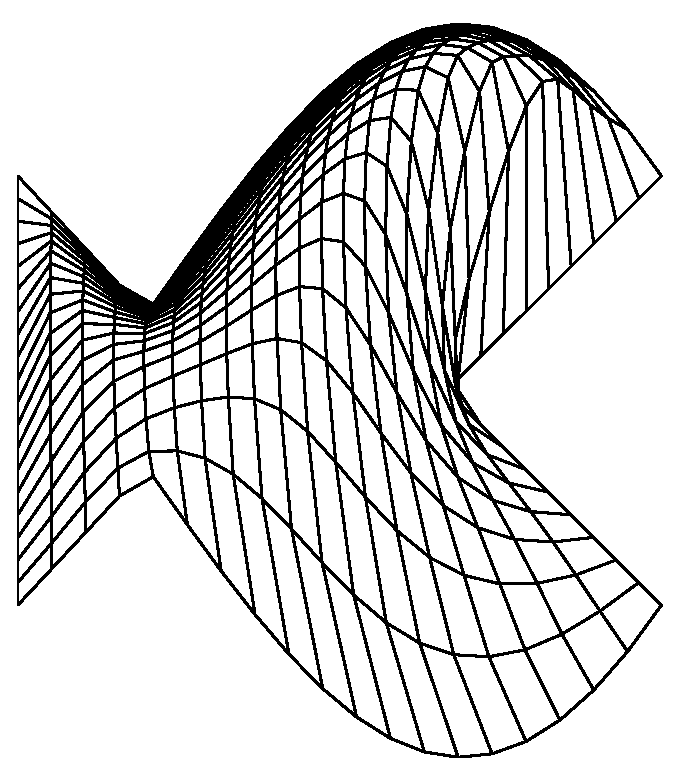
\includegraphics[width=0.7\textwidth]{figures/fish-ttm-sor.eps}
				\caption{SOR - 71 iterações}
			\end{subfigure}
			\caption{Domínio Peixe, aplicando o método TTM para aproximação para a linha $\xi = 1$}
			\label{fig:fish:ttm:}
			\centering
			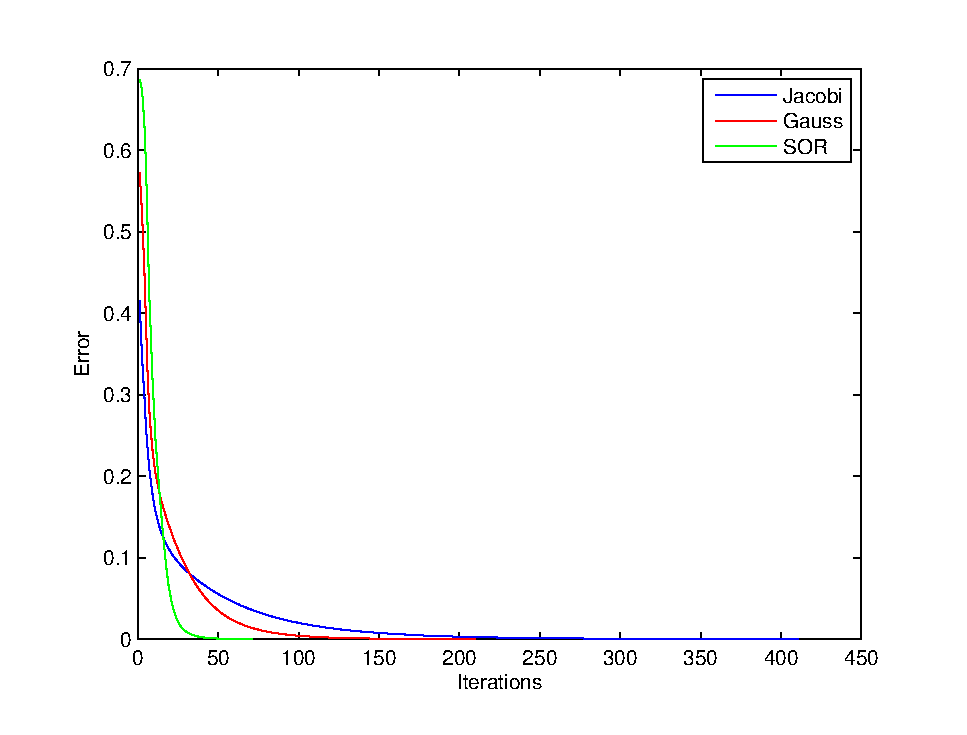
\includegraphics[width=0.7\textwidth]{figures/fish-ttm-error.eps}
			\caption{Gráfico do erro para o domínio peixe com aproximação em linha}
			\label{fig:fish:ttm:erro}
		\end{figure}

		\begin{figure}
		\centering
			\begin{subfigure}[b]{0.45\textwidth}
				\centering
				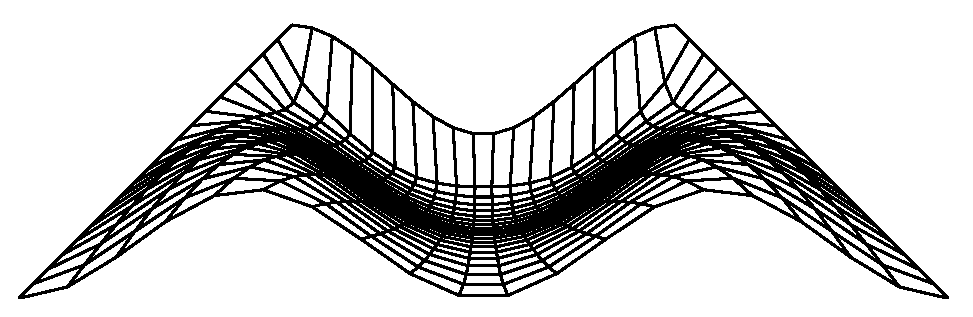
\includegraphics[width=\textwidth]{figures/m-ttm-jacobi.eps}
				\caption{Jacobi - 1875 iterações}
			\end{subfigure}
			\begin{subfigure}[b]{0.45\textwidth}
				\centering
				\includegraphics[width=\textwidth]{figures/m-ttm-gauss.eps}
				\caption{Gauss-Seidel - 119 iterações}
			\end{subfigure}
			\begin{subfigure}[b]{0.45\textwidth}
				\centering
				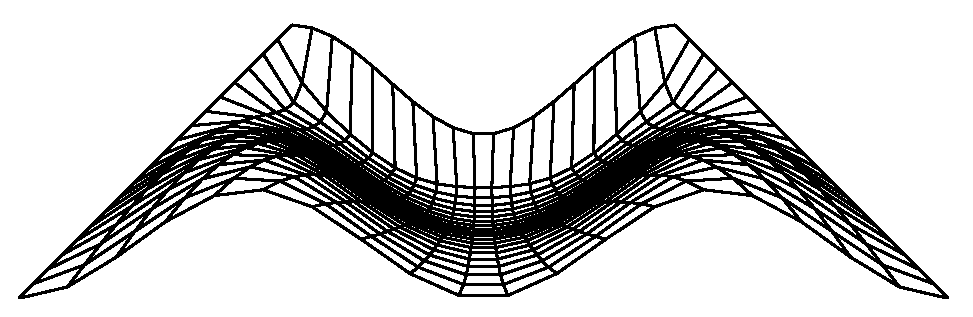
\includegraphics[width=\textwidth]{figures/m-ttm-sor.eps}
				\caption{SOR - 447 iterações}
			\end{subfigure}
			\caption{Domínio M, aplicando o método TTM para aproximação para o ponto (0.5,0.5)}
			\label{fig:m:ttm}
			\centering
			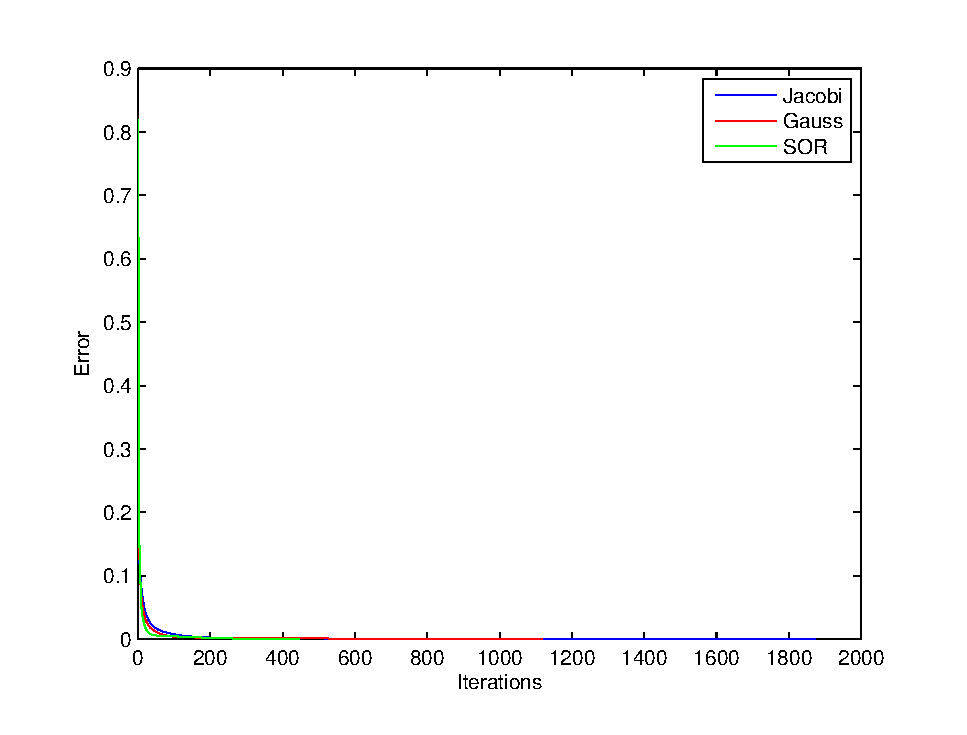
\includegraphics[width=0.7\textwidth]{figures/m-ttm-error.eps}
			\caption{Gráfico do erro para o domínio M com aproximação pontual}
			\label{fig:m:ttm:erro}
		\end{figure}
	% section resultados (end)
	
	\section{Considerações Finais} % (fold)
	\label{sec:considera_es_finais}
		É possível notar que a adaptividade da malha pode ajudar em vários casos onde é necessário mais detalhes em regiões específicas. Com a técnica TTM é possível obter boas malhas com segurança de respeito ao domínio imposto.

		Vale ressaltar que a amplitude escolhida nos casos relatados foi exaustivamente testada. Em casos extremos, é possivel degenerar a malha, levando a resultados muito ruins. O bom senso na escolha da amplitude se faz necessário, evitando-se assim valores muito extremos.
	% section considera_es_finais (end)

	\bibliography{/home/rnakanishi/Documents/latex/refs.bib}
	\bibliographystyle{acm}
\end{document}
